% 完整编译: XeLaTex -> BibTex -> XeLaTex -> XeLaTex

%%%%%%%%%%%%%%%%%%%%%%%%  文档配置  %%%%%%%%%%%%%%%%%%%%%%%%

\documentclass[report, twoside, UTF8, AutoFakeBold = 1, AutoFakeSlant, zihao = -4]{config}

% 封面图片定义
\def \titlePageImages{
    
\includegraphics[width=0.45\textwidth] {NWPU-logo.pdf}\\ % 校徽
    
\includegraphics[width=0.45\textwidth] {NWPU-title-CN.pdf}\\ % 中文校名
    
\includegraphics[width=0.55\textwidth] {NWPU-title-EN.pdf}\\ % 英文校名    
}

% 文档信息定义
\def \majorTitle   {模板使用指南} % 大标题
\def \minorTitleCN {基于 \LaTeX{} 的论文/报告/作业模板(非官方)使用指南} % 中文标题
\def \minorTitleEN {\LaTeX{}-based Thesis/Report/Assignment Template (Not Official) User Guide} % 英文标题
\def \currentDate  {\zhtoday} % 日期 \zhtoday获取当前中文日期

\def \classificationNumber  {A0001} % 分类号
\def \UDC                   {} % UDC
\def \confidentialLevel     {公开} % 密级
\def \serialNumber          {0001} % 编号

% 个人信息定义
\def \titlePageInfoBox{
    % 参数:#1下划线长度 #2字号 #3标题 #4内容
    \infobox{6cm}{-2}{版~~~~~~~~本}{v1.0}\\
    \infobox{6cm}{-2}{学~~~~~~~~院}{摸鱼学院}\\
    \infobox{6cm}{-2}{专~~~~~~~~业}{摸鱼科学与技术}\\
    \infobox{6cm}{-2}{班~~~~~~~~级}{阿巴阿巴}\\
    \infobox{6cm}{-2}{姓~~~~~~~~名}{Sugar}\\
    \infobox{6cm}{-2}{学~~~~~~~~号}{114514}\\
    \infobox{6cm}{-2}{指导教师}{无师自通}\\
}

%%%%%%%%%%%%%%%%%%%%%%%%  文档开始  %%%%%%%%%%%%%%%%%%%%%%%%

\begin{document}

% 封面
\CoverPage
    {empty} % 封面类型:both、left、right、empty
    {1} % 大标题字号
    {2} % 中文标题字号
    {-2} % 英文标题字号

%%%%%%%%%%%%%%%%%%%%%  正文前页眉页脚  %%%%%%%%%%%%%%%%%%%%%%

% 页眉(关闭页眉务必将页眉类型设为empty)
\Header
    {common} % 页眉类型:common、publish、empty
    {1pt} % 上分隔线宽度
    {1pt} % 两线距离
    {0.5pt} % 下分割线宽度
    {} % 页眉左自定义内容(文本或图片)
    {
\includegraphics[width=0.15\textwidth]{NWPU-title-CN.pdf}} % 页眉中自定义内容(文本或图片)
    {} % 页眉右自定义内容(文本或图片)

%============================================%

% 页脚(关闭页脚务必将页脚类型设为empty) 
\Footer
    {common} % 页脚类型:common、publish、empty
    {0pt} % 上分隔线宽度
    {0pt} % 两线距离
    {0pt} % 下分割线宽度
    {} % 页脚左自定义内容(文本或图片)
    {\thepage} % 页脚中自定义内容(文本或图片)
    {} % 页脚右自定义内容(文本或图片)

%============================================%

% 页数样式 参数:#1起始页数
\SetRomanPageNumber{1} % 设置罗马数字页码
% \setArabicPageNumber{1} % 设置阿拉伯数字页码

%%%%%%%%%%%%%%%%%%%%%%%%  摘要  %%%%%%%%%%%%%%%%%%%%%%%

\begin{abstractCN}[-2] % 中文摘要,参数:#1中文摘要标题字号

\LaTeX{}(发音为 “Lah-tech” 或 “Lay-tech” )是由 Leslie Lamport 开发的当今世界上最流行和使用最为广泛的 \TeX{} 宏集。它构筑在 PlainTeX 的基础之上,并加进了很多的功能以使得使用者可以更为方便的利用 \TeX{} 的强大功能。

使用 \LaTeX{} 基本上不需要使用者自己设计命令和宏等,因为 \LaTeX{} 已经替你做好了。因此,即使使用者并不是很了解 \TeX{},也可以在短短的时间内生成高质量的文档。对于生成复杂的数学公式,\LaTeX{} 表现的更为出色。

\LaTeX{} 由 \LaTeX{3} 项目维护,很多使用者对 \LaTeX{} 加入了很多补充扩展,例如为 \LaTeX{} 开发宏包和样式,其中的一些已经包含在很多 \LaTeX{} 软件中,可以在CTAN上获得更多的扩展宏包。

% 中文关键词
\def\keywordsCN{关键词1,关键词2,关键词3,关键词4,关键词5}

\end{abstractCN}

%============================================%

\begin{abstractEN}[-2] % 英文摘要,参数:#1英文摘要标题字号

\LaTeX{} (pronounced either ``Lah-tech" or ``Lay-tech") is a set of macros for \TeX{} created by Leslie Lamport. Its purpose is to simplify \TeX{} typesetting, especially for documents containing mathematical formulae. Within the typesetting system, its name is formatted as ``\LaTeX{}".

\TeX{} is both a typographical and a logical markup language, and one has to take account of both issues when writing a \TeX{} document. On the other hand, Lamport's aim when creating \LaTeX{} was to split those two aspects. A typesetter can make a template and then the writers can just focus on \LaTeX{} logical markup. They might not know anything about typesetting.

In addition to the commands and options \LaTeX{} offers, many other authors have contributed extensions, called packages or styles, which you can use for your documents. Many of these are bundled with most \TeX{}/\LaTeX{} software distributions; more can be found in the Comprehensive \TeX{} Archive Network (CTAN).

% 英文关键词
\def\keywordsEN{keyword 1,keyword 2,keyword 3,keyword 4,keyword 5}

\end{abstractEN}

%%%%%%%%%%%%%%%%%%%%%%%  启用目录  %%%%%%%%%%%%%%%%%%%%%%%%

\contentPage{1.5}{目~~~~录}            % 总目录,参数:#1目录行距 #2目录标题
\contentpageOfFigures{1.5}{图目录}     % 图目录,参数:#1目录行距 #2目录标题
\contentpageOfTables{1.5}{表目录}      % 表目录,参数:#1目录行距 #2目录标题

%%%%%%%%%%%%%%%%%%%%%%%  启用水印  %%%%%%%%%%%%%%%%%%%%%%%%

\imageWatermark % 图片水印
    {0} % 旋转角度
    {0.8} % 放缩倍率
    {0.02} % 透明度 在0-1之间调整
    {NWPU-logo.eps} % 图片路径

%%%%%%%%%%%%%%%%%%%%%  正文页眉页脚  %%%%%%%%%%%%%%%%%%%%%%

% 页眉(关闭页眉务必将页眉类型设为empty)
\Header
    {common} % 页眉类型:common、publish、empty
    {1pt} % 上分隔线宽度
    {1pt} % 两线距离
    {0.5pt} % 下分割线宽度
    {使用指南} % 页眉左自定义内容(文本或图片)
    {} % 页眉中自定义内容(文本或图片)
    {\currentChapterInfo} % 页眉右自定义内容(文本或图片)

%============================================%

% 页脚(关闭页脚务必将页脚类型设为empty) 
\Footer
    {common} % 页脚类型:common、publish、empty
    {0pt} % 上分隔线宽度
    {0pt} % 两线距离
    {0pt} % 下分割线宽度
    {} % 页脚左自定义内容(文本或图片)
    {\thepage} % 页脚中自定义内容(文本或图片)
    {} % 页脚右自定义内容(文本或图片)

%============================================%

% 页数样式 参数:#1起始页数
% \setRomanPageNumber{1} % 设置罗马数字页码
\SetArabicPageNumber{1} % 设置阿拉伯数字页码

%%%%%%%%%%%%%%%%%%%%%%%  正文  %%%%%%%%%%%%%%%%%%%%%%%%%%

\chapter{关于本模板}

\section{介绍}

\LaTeX{} 是一个强大的文档排版工具,但其相对较大的学习成本往往让初学者难以上手使用。为了让初学者能轻松使用 \LaTeX{},作者通过对一些成熟的方案进行整合、封装,创作出本模板,但由于作者水平有限,模板中仍存在一些不足,作者将会尽力修改完善。

本使用指南演示了模板中的一些典型使用场景,其中包括:

\begin{itemize}
    \item \textbf{排版相关:}封面页、页眉页脚、目录样式、标题样式、图表样式、脚注等。
    \item \textbf{文本相关:}多级标题、列表。
    \item \textbf{图表相关:}单个图片、多个图片。普通表格、复杂表格、跨页表格。
    \item \textbf{引用相关:}多种样式的文献引用。
    \item \textbf{数学相关:}数学符号、公式、定理证明。
    \item \textbf{代码相关:}算法(伪代码)、代码块。
\end{itemize}

作者在开发本模板时大量参考、模仿、学习了许多优秀的第三方模板,参考的内容和参考模板的地址如表 \ref{tab:templates} 所示。

\begin{table}
    \centering
    \renewcommand{\arraystretch}{1.2} % 定义表格行距
    \setlength{\tabcolsep}{3pt} % 定义列间宽度
    \caption{参考模板相关信息}
    \label{tab:templates}
    \begin{threeparttable}[c]
        \begin{tabular}{ccc}
            \toprule[1.5pt]
            \textbf{参考模板}    &  \textbf{参考内容}    & \textbf{模板地址}\\
            \midrule[0.8pt]
            清华大学学位论文模板 & 示例文档、部分模板源码 & \href{https://github.com/tuna/thuthesis}{Github 地址}\\
            华南师范大学本科毕业论文模板 & 部分模板源码 & \href{https://www.overleaf.com/latex/templates/scnu-my-article/jkbbvhnddtsw}{OverLeaf 地址}\\
            上海师范大学研究生毕业论文模板 & 部分模板源码 & \href{https://www.overleaf.com/latex/templates/shnu-thesis/wsykzrksspgn}{OverLeaf 地址}\\
            武汉大学博士论文模板 & 部分模板源码 & \href{https://www.overleaf.com/latex/templates/wu-yi-da-xue-bo-shi-lun-wen-latex-mo-ban/rcdzgvqgkddk}{OverLeaf 地址}\\
            南开大学毕业论文模板 & 部分模板源码 & \href{https://github.com/Tr0py/NKU-thesis-template-2020}{Github 地址}\\
            复旦大学博士学位论文模板 & 部分模板源码 & \href{https://cn.overleaf.com/latex/templates/fduthesis-latex-thesis-template-for-fudan-university/svtdhhstkmkt}{OverLeaf 地址}\\
            \bottomrule[1.5pt]
        \end{tabular}
    \end{threeparttable}
\end{table}

\section{协议}

本模板采用 LPPL v1.3c\footnote{\url{https://www.latex-project.org/lppl/lppl-1-3c/}}或其之后的版本进行许可,请在遵循许可的前提下使用本模板。

\section{模板文件结构}

本模板的文件目录结构如表 \ref{tab:文件目录} 所示。

\begin{table}
  \centering
  \caption{模板文件目录结构}
  \label{tab:文件目录}
  % \renewcommand\arraystretch{1.2} % 定义表格行距
  \setlength{\tabcolsep}{30pt} % 定义列间宽度
  \begin{tabular}{ll}
    \toprule[1.5pt]
    \textbf{文件名}           & \textbf{说明}\\
    \midrule[0.8pt]
    fonts                    & 字体文件夹\\
    images                   & 图片文件夹\\
    config.cls               & 模板文件\\
    \textbf{guide.tex}       & \textbf{使用指南文本文件}\\
    License                  & 软件许可证文件\\
    \textbf{main.tex}        & \textbf{空白文本文件}\\
    references.bib           & 参考文献表样式文件\\
    \bottomrule[1.5pt]
  \end{tabular}
\end{table}

其中,.cls 文件中定义了宏包、指令等,可以大致理解为模板的配置文件、源代码文件;.tex 文件用于编写主要的文本内容;.bib 文件是 \hologo{BibTeX} 所使用的文件,用于存放引用文献的相关信息。

\file{fonts} 文件夹用于存放模板中用到的字体。\file{images} 文件夹用于存放模板中用到的图片,\file{images/logos} 文件夹中存放的图片被用于封面页和水印。

\section{模板使用方式}

因本模板的所有编写都在 OverLeaf\footnote{OverLeaf 是一个强大的线上编辑 \LaTeX{} 文档工具,提供实时预览、线上存储、多人协作、版本管理、模板分享等功能。} 上完成,所以本文仅介绍模板在 OverLeaf 上的使用方法。

要在 OverLeaf 上使用本模板,只需要将模板的 rar 压缩文件上传至 OverLeaf 的个人项目库中打开即可。使用模板时,务必保证使用的编译器为 \hologo{XeLaTeX}。

熟悉本模板以及 \LaTeX{} 的基本操作后,建议将主文档文件切换为 \file{main.tex} 直接使用。

\chapter{文本相关}

本章节介绍使用 \LaTeX{} 完成简单的文本操作,其中包括分级标题、段落、列表(部分功能)的使用演示。文本内容选取自 \LaTeX{} 的维基教科书介绍\footnote{\url{https://en.wikibooks.org/wiki/LaTeX/Introduction}}。

\section{了解 \TeX{}}

\TeX{}(X 或 $\chi$)是由 Donald Knuth 创造的基于低级编程语言的电子排版系统,利用 \TeX{} 能够对文章进行十分精美的排版。\TeX{} 提供了一套功能强大并且十分灵活的排版语言,它多达 900 多条指令,支持 if-else 判断语句和运算(运算在文档编译的过程中执行)等功能,并且 \TeX{} 有宏功能,用户可以不断地定义自己适用的新命令来扩展 \TeX{} 系统的功能。许多人利用 \TeX{} 提供的宏定义功能对 \TeX{} 进行了二次开发,其中比较著名的有美国数学学会(AMS)推荐的非常适合于数学家使用的 \hologo{AmSLaTeX} 以及适合于一般文章、报告、书籍的 \LaTeX{} 系统。

\TeX{} 系统是公认的数学公式排得最好的系统。美国数学学会鼓励数学家们使用 \TeX{} 系统向它的期刊投稿。世界上许多一流的出版社如 Kluwer、Addison-Wesley、牛津大学出版社等也利用 \TeX{} 系统出版书籍和期刊。

\TeX{} 的强大之处在于其能够对文档的排版进行非常精细的操作,但也会造成难度的提高和耗时增加。1977 年,随着数字印刷的逐步发展,Donald Knuth 发现了数字印刷的潜力并开始 \TeX{} 排版引擎的编写工作,以改善日益恶化的印刷质量。我们现在用的 \TeX{} 排版系统发布于 1982 年,在 1989 年为了更好地支持多国语言又进行了一些改进。\TeX{} 具有很好的稳定性,能够在许多不同种类的计算机上运行,几乎不出现错误。

\TeX{} 一词来源于希腊语“τεχνολογία”(“technologìa”),意为“科技”;它的第一个音节“τεχ”与“TEX”相似,因此英文名取作“TEX”。\TeX{} 系统以逐渐收敛到 $\pi$ 的数字作为版本号。

\section{了解 \LaTeX{}}

\LaTeX{}(发音为“Lah-tech”或“Lay-tech”)是由 Leslie Lamport 开发的当今世界上最流行和使用最为广泛的 \TeX{} 宏集。它构筑在 PlainTeX 的基础之上,并加进了很多的功能以使得使用者可以更为方便的利用 \TeX{} 的强大功能。使用 \LaTeX{} 基本上不需要使用者自己设计命令和宏等,因为 \LaTeX{} 已经替你做好了。因此,即使使用者并不是很了解 \TeX{},也可以在短短的时间内生成高质量的文档。对于生成复杂的数学公式,\LaTeX{} 表现的更为出色。\LaTeX{} 由 \LaTeX{3} 项目维护,很多使用者对 \LaTeX{} 加入了很多补充扩展,例如为 \LaTeX{} 开发宏包和样式,其中的一些已经包含在很多 \LaTeX{} 软件中,可以在 CTAN 上获得更多的扩展宏包。

\subsection{\LaTeX{} 的缺点}

% 无序列表
\begin{itemize}
    \item 一般来说是不能在输入文章的同时看到最终的输出效果,但是将文章用 \LaTeX{} 编译之后,是可以在屏幕上预览最终的输出效果的。尽管在预先定义好的版面中可以调节一些参数,设计全新的版面还是很困难的,需要耗费大量的时间。
    \item 尽管在预先定义好的版面中可以调节一些参数,设计全新的版面还是很困难的,需要耗费大量的时间。
    \item 需要掌握一些 \LaTeX{} 的排版命令。
    \item \LaTeX{} 不适合于排版非结构化的、无序的文档。
\end{itemize}

\subsection{\LaTeX{} 的优点}

% 有序列表
\begin{enumerate}
    \item 提供专业级的排版设计,使你的文档看起来如同印刷好的一样。
    \item 可以更方便地排版数学公式。
    \item 用户仅仅需要掌握少数容易理解的,用来说明文档逻辑结构的命令,而无需对实际的页面设计做胡乱的修补。
    \item 可以很容易地生成脚注、索引、目录和参考文献等复杂的结构。
    \item 有大量免费的可添加宏包,协助你完成许多基本的 \LaTeX{} 未直接支持的排版任务。例如,支持在文档中插入PostScript图形的宏包和排版符合各类标准的参考文献的宏包等。
    \item \LaTeX{} 支持DVI和PDF格式的输出,如配合其他软件可以很容易地生成 PostScript、PNG、JPG 等格式的输出。
    \item 有大量免费的可添加宏包,协助你完成许多基本的 \LaTeX{} 未直接支持的排版任务。例如,支持在文档中插入 PostScript 图形的宏包和排版符合各类标准的参考文献的宏包等。
    \item \TeX{} 作为 \LaTeX{} 的格式化引擎,是免费软件并且具有极高的可移植性,因此它几乎可以在任何硬件平台上运行。
\end{enumerate}

\chapter{图表相关}

\section{图片}

\subsection{单个图片}

图片通常在 figure 环境中使用 includegraphics 插入,如图 \ref{fig:example1} 的源代码。建议使用矢量图片(PDF)。照片建议使用 JPG 格式。其他的栅格图建议使用无损的 PNG 格式。

\begin{figure}[H] % 图片位置固定
    \centering % 图片居中
    \includegraphics{example-image} % 图片路径
    \caption*{图片的说明文字。} % 图片说明文字
    \caption{图片的标题} % 图片标题
    \label{fig:example1} % 图片标签
\end{figure}

图片可以通过 width 参数来设置宽度,设置宽度后长度会等比例放缩。一般 width 参数会搭配 \cs{linewidth} 使用,以实现按照当前页面宽度进行等比例放缩。使用的效果如图 \ref{fig:example2} 所示。

\begin{figure}[H]
    \centering
    \includegraphics[width=0.5\linewidth]{example-image}
    \caption{一张缩小到当前页宽的 0.5 倍的图片}
    \label{fig:example2}
\end{figure}

\clearpage

使用 \pkg{tikz} 宏包可以直接画图,该宏包的学习成本极高,不建议初学者使用。以下图片是 \pkg{tikz} 的一些使用案例。

\begin{figure}[H]
    \centering
    \resizebox{0.95\columnwidth}{!}{
        \tikzstyle{information text}=[text badly centered,font=\small,text width=3cm]
\begin{tikzpicture}[scale=.6,cap=round]
    % The graphic
    \begin{scope}[>=stealth', line width=1pt]
        \draw[->] (1,.9) node[below, information text]
            {Phonological representation of root form } -- (1,1.8);
        \draw[->] (5,-.2) node[below,information text]
            {Wickelfeature representation of root form } -- (5,.8);
        \draw[->] (11,-.2) node[below,information text]
            {Wickelfeature representation of past tense } -- (11,.8);
        \draw[->] (16,0.9) node[below,information text]
            {Phonological representation of past tense } -- (16,1.8);
    \end{scope}
    \draw (3,6) node[information text] { Fixed Encoding Network };
    \draw (8,6) node[information text, text width=4cm, ]
        { Pattern Associator Modifiable Connections };
    \draw (13.5,6) node[information text] { Decoding/Binding Network };
    % draw the nodes
    \foreach \x in {1,16}
        \foreach \y in {2,3,4} {
        \filldraw[fill=white] (\x,\y) circle (0.1);
        }
    \foreach \x in {5,11}
        \foreach \y in {1,2,3,4,5} {
            \filldraw[fill=white] (\x,\y) circle (0.1);
        }
    % The lines connecting the nodes are drawn in the background layer.
    % This way we can hide the lines behind the nodes and don't worry
    % about the width of each node.    
    \begin{pgfonlayer}{background}
        % we add the lines for the nodes starting in y 2,3, and 4
        \foreach \xa / \xb in {1 / 5, 5 / 11 , 11 / 5 , 16 / 11}
            \foreach \ya / \yb / \yc / \yd / \ye in {2 / 3 / 4 / 5 / 1, 
            3 / 4 / 5 / 1 / 2, 4 / 5 / 1 / 2 / 3} {
                \draw (\xa,\ya) -- (\xb,\ya);
                \draw (\xa,\ya) -- (\xb,\yb);
                \draw (\xa,\ya) -- (\xb,\yc);
                \draw (\xa,\ya) -- (\xb,\yd);
                \draw (\xa,\ya) -- (\xb,\ye);
            }
        % add remaining lines from y1 to y5
        \foreach \xa / \xb in {5 / 11 , 11 / 5}
            \foreach \ya / \yb in {1 / 5, 5 / 1} {
            \draw (\xa,\ya) -- (\xb,\ya);
            \draw (\xa,\ya) -- (\xb,\yb);
        }
    \end{pgfonlayer}
\end{tikzpicture}
    }
    \caption{神经网络示意图}
    \label{fig:neural network example}
\end{figure}

\begin{figure}[H]
    \centering
    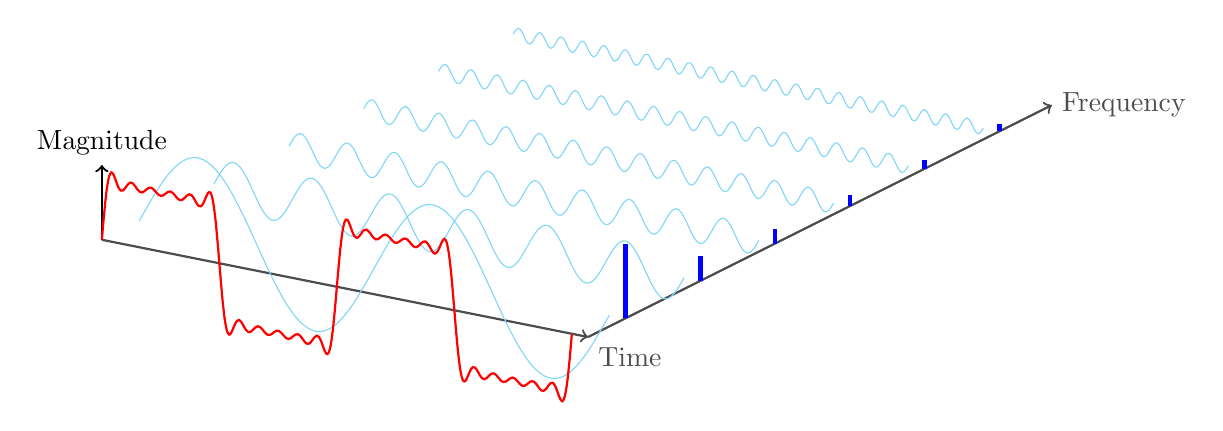
\begin{tikzpicture}[x={(1cm,0.5cm)},z={(0cm,0.5cm)},y={(1cm,-0.2cm)},scale=0.95]
    \draw[->,thick,black!70] (0,6.5,0) -- (6.2,6.5,0) node[right] {Frequency}; % 频率轴
    \draw[->,thick,black!70] (0,0,0) -- (0,6.5,0) node[below right] {Time}; % 时间轴
    \draw[->,thick] (0,0,0) -- (0,0,2) node[above] {Magnitude}; 
    
    \foreach \n in {0.5,1.5,...,5.5}{
    \draw [cyan!50, domain=0:2*pi,samples=200,smooth] 
     plot (\n,\x, {sin(4*\n*\x r)/\n });
    \draw[blue, ultra thick] (\n,6.5,0) -- (\n,6.5,1/\n);
    } % 频率逐渐增大振幅逐渐变小的正弦函数
    
    \draw [red, thick, domain=0:2*pi,samples=200,smooth] 
    plot (0,\x, {sin(4*0.5*\x r)/0.5 + sin(4*1.5*\x r)/1.5 + sin(4*2.5*\x r)/2.5 + sin(4*3.5*\x r)/3.5 + sin(4*4.5*\x r)/4.5 + sin(4*5.5*\x r)/5.5} ); 
    % 最后是手动加起来得到矩形波的逼近
\end{tikzpicture}

    \caption{波的叠加示意图} 
    \label{fig:superposition of waves}
\end{figure}

\begin{figure}[H]
    \centering
    \resizebox{1\columnwidth}{!}{
         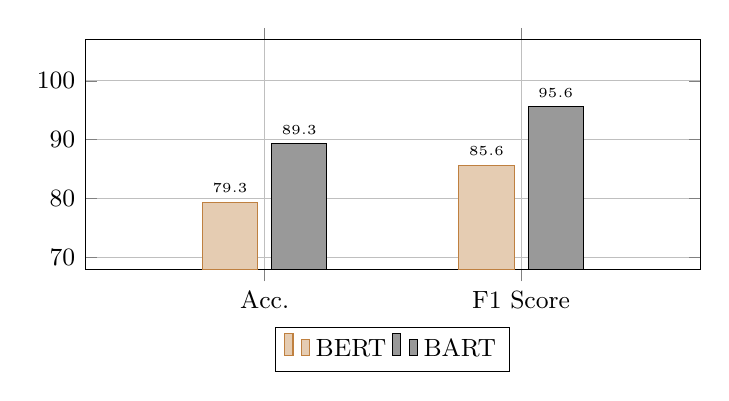
\begin{tikzpicture} 
 \begin{axis}[
 enlargelimits=0.7,
 legend style={at={(0.5,-0.25)},
  anchor=north,legend columns=-1},
 symbolic x coords={Acc., F1 Score },
 xtick=data,
 ybar=5pt,% configures `bar shift'
 bar width=20pt,
 width=9.4cm, height=4.5cm,
 nodes near coords,
 nodes near coords align={vertical},
 nodes near coords style={font=\tiny},
 font=\small,
 grid=major,
 ]
 \addplot[fill=brown!40!white,draw=brown] coordinates {
  (Acc., 79.3)
  (F1 Score, 85.6)
 };
 \addplot [fill=black!40!white,draw=black] coordinates {
  (Acc., 89.3)
  (F1 Score, 95.6)
 };
 \legend{BERT, BART}
 \end{axis}
 \end{tikzpicture}
    }
    \caption{柱状图} 
    \label{fig:histogram}
\end{figure}

\begin{figure}[H]
    \centering
    \resizebox{1\columnwidth}{!}{
        \definecolor{color1}{RGB}{145,30,180}
\definecolor{color2}{RGB}{245,130,48}
\definecolor{color3}{RGB}{230,25,75}

\begin{tikzpicture}
\footnotesize
\scalefont{0.7} %设置字体大小
\begin{axis}[
width=8cm, height=5cm,  %设置长和宽
ymin=30, ymax=80,
ytick={30,45,60,75},
ylabel style={text width=0.3\columnwidth,align=center}, 
xlabel= x,
ylabel = y,
width=0.6\columnwidth, 
xmin=0,xmax=20,
xtick={0,5,10,15,20},
ylabel near ticks,
legend style={at={(0.9,1.1)},anchor=south},
]

% 下界1
\addplot[draw=none,mark=none,name path=SeqSeqOneLower,forget plot] coordinates{
(0,64.62)
(5,33.03)
(10,35.30)
(15,34.03)
(20,34.32)
 };
% 上界1    
 \addplot[draw=none,mark=none,name path=SeqSeqOneUpper,forget plot] coordinates{
(0,68.54)
(5,38.40)
(10,42.67)
(15,38.59)
(20,50.05)
 };     
%下界1与上界1之间填充
\addplot [fill=color1,opacity=0.2,forget plot] fill between[of=SeqSeqOneLower and SeqSeqOneUpper];
% 绘制折线1     
 \addplot[color=color1,style={ thick}] coordinates { 
 (0,66.58)
(5,35.71)
(10,38.99)
(15,36.31)
(20,42.19)
}; 
\addlegendentry{\textsc{a}} % 设置名称1
      
% 下界2          
 \addplot[draw=none,mark=none,name path=SeqSeqLower,forget plot] coordinates{
(0,69.19)
(5,49.82)
(10,48.77)
(15,46.94)
(20,44.27)
};
% 上界2 
\addplot[draw=none,mark=none,name path=SeqSeqUpper,forget plot] coordinates{
(0,74.39)
(5,51.66)
(10,57.90)
(15,66.40)
(20,63.23)
};     
%下界2与上界2之间填充     
\addplot [fill=color2,opacity=0.2,forget plot] fill between[of=SeqSeqLower and SeqSeqUpper];
% 绘制折线2
\addplot[color=color2,style={ thick}] coordinates { 
(0,71.79)
(5,50.74)
(10,53.33)
(15,56.67)
(20,53.75)
}; 
\addlegendentry{\textsc{b}}
     
% 下界3    
\addplot[draw=none,mark=none,name path=FullGoldLower,forget plot] coordinates{
(0,71.57)
(5,62.72)
(10,55.14)
(15,57.42)
(20,62.86)
};
% 上界3     
\addplot[draw=none,mark=none,name path=FullGoldUpper,forget plot] coordinates{
(0,73.49)
(5,65.95)
(10,62.96)
(15,70.2)
(20,79.64)
 };     
%下界3与上界3之间填充    
\addplot [fill=color3,opacity=0.2,forget plot] fill between[of=FullGoldLower and FullGoldUpper];
% 绘制折线3
\addplot[color=color3,style={ thick}] coordinates { 
(0,72.53)
(5,64.33)
(10,59.05)
(15,63.81)
(20,71.25)
}; 
\addlegendentry{\textsc{c}}
        
\end{axis}

\end{tikzpicture}
    }
    \caption{带误差的折线图} 
    \label{fig:line chart with error bar}
\end{figure}

\begin{figure}[H]
    \centering
    \resizebox{1\columnwidth}{!}{
        % 这里将第一年yearOne设置为图中起始年,后续就可以直接用年月的形式2019.05直接定义节点的位置
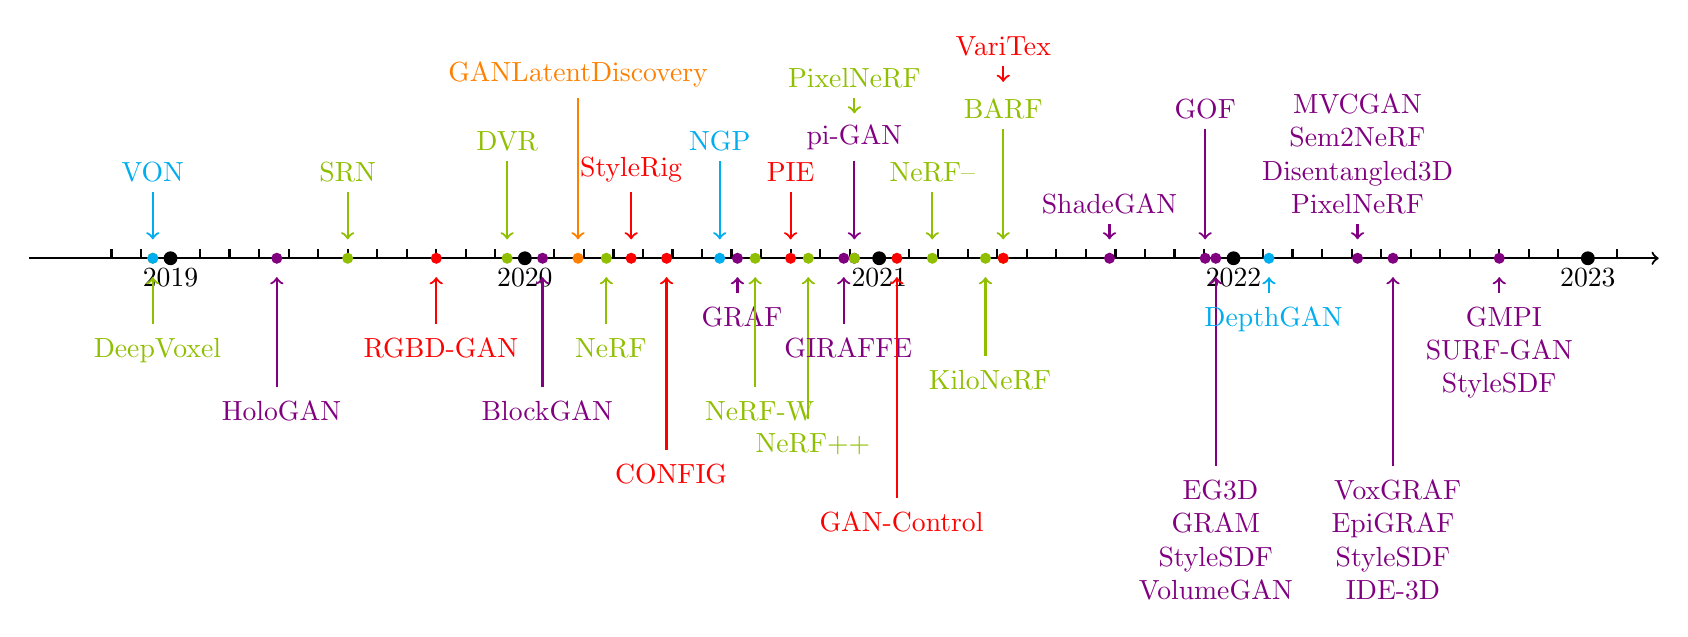
\begin{tikzpicture}%
  \newcount\yearOne; 
  \yearOne= 2019 
  \def\n{4}
  \def\w{18}  
  \def\lt{0.40} 
  \def\lf{0.36} 
  \def\lo{0.12} 
  \def\lext{0.1} 
  \def\rext{1.05} 
  \def\yearLabel(#1,#2,#3){\node[above,black!60!cyan] at ({(#1-\yearOne)*\w/\n},{\lt*#2}) {#3};}

% define yearArrowLabel (#position, #arrow direction(up/down), #arrow length, #method, #color)
    \def\yearArrowLabel(#1,#2,#3,#4,#5){
    \def\xy{{(#1-\yearOne)*\w/\n}}; \pgfmathparse{int(#2*100)};
    \ifnum \pgfmathresult<0 %
      \def\yyp{{(\lt*(0.90+#2))}}; \def\yyw{{(\yyp-\lt*#3)}}
      \fill[color=#5,radius=2pt] (\xy,0) circle;
      \draw[<-,thick,color=#5,align=center]
        (\xy,\yyp) -- (\xy,\yyw)
        node[below,color=#5] at (\xy,\yyw) {\strut #4};
    \else %
      \def\yyp{{(\lt*(0.10+#2)}}; \def\yyw{{(\yyp+\lt*#3)}}
      \fill[color=#5,radius=2pt] (\xy,0) circle;
      \draw[<-,thick,color=#5,align=center]
        (\xy,\yyp) -- (\xy,\yyw)
        node[above] at (\xy,\yyw) {#4};
    \fi}
    
    \draw[->,thick] (-\w*\lext,0) -- (\w*\rext,0);
    
    \foreach \tick in {0,1,...,\n}{
      \def\x{{\tick*\w/\n}}
      \def\year{\the\numexpr \yearOne+\tick*1 \relax}
      \fill[black,radius=2.5pt] (\x,0) circle;
      \draw[thick] (\x,-0.0001) -- (\x,0.0001) %
	               node[below] {\year};
      \ifnum \tick<\n
        \foreach \ticko in {1,2,3,4,5,6,7,8,9,10,11}{
          \def\xo{{(\x+\ticko*\w/\n/12)}}
  	      \draw[thick] (\xo,0) -- (\xo,\lo);  %
	  }\fi
    }
    \draw[thick] (-1*\w/\n/12,0) -- (-1*\w/\n/12,\lo);
    \draw[thick] (-2*\w/\n/12,0) -- (-2*\w/\n/12,\lo);
    \draw[thick] ({\w+\w/\n/12},0) -- ({\w+\w/\n/12},\lo);
  
    \yearArrowLabel(2018.95,-1.5,1.5, DeepVoxel, black!25!lime)  %
    \yearArrowLabel(2018.95,0.5,1.5,VON, cyan)          
    \yearArrowLabel(2019.30,-1.5,3.5, HoloGAN, violet)  %
    \yearArrowLabel(2019.50,0.5,1.5, SRN, black!25!lime) 
    \yearArrowLabel(2019.75,-1.5,1.5, RGBD-GAN, red) 
    \yearArrowLabel(2019.95,0.5,2.5, DVR, black!25!lime) 
    \yearArrowLabel(2020.05,-1.5,3.5, BlockGAN, violet) 
    \yearArrowLabel(2020.15,0.5,4.5, GANLatentDiscovery, orange)
    \yearArrowLabel(2020.23,-1.5,1.5, NeRF, black!25!lime)
    \yearArrowLabel(2020.30,0.5,1.5, StyleRig, red) 
    \yearArrowLabel(2020.40,-1.5,5.5, CONFIG, red) 
    \yearArrowLabel(2020.55, 0.5,2.5, NGP, cyan)   %
    \yearArrowLabel(2020.60,-1.5,0.5, GRAF, violet)  %
    \yearArrowLabel(2020.65,-1.5,3.5, NeRF-W, black!25!lime) 
    \yearArrowLabel(2020.75,0.5,1.5, PIE, red) 
    \yearArrowLabel(2020.80,-1.5,4.5, NeRF++, black!25!lime) 
    \yearArrowLabel(2020.90,-1.5,1.5, GIRAFFE, violet) 
    \yearArrowLabel(2020.93,0.5,2.5, pi-GAN, violet) 
    \yearArrowLabel(2020.93,4.5,0.5, PixelNeRF, black!25!lime) 
    \yearArrowLabel(2021.05,-1.5,7.0, GAN-Control, red)
    \yearArrowLabel(2021.15,0.5,1.5, NeRF--, black!25!lime) 
    \yearArrowLabel(2021.30,-1.5,2.5, KiloNeRF, black!25!lime) 
    \yearArrowLabel(2021.35,0.5,3.5, BARF, black!25!lime) 
    \yearArrowLabel(2021.35,5.5,0.5, VariTex, red) 
    \yearArrowLabel(2021.65,0.5,0.5, ShadeGAN, violet)
    \yearArrowLabel(2021.92, 0.5,3.5, GOF, violet) 
    \yearArrowLabel(2021.95, -1.5, 6.0, EG3D\\GRAM\\StyleSDF\\VolumeGAN, violet) 
    \yearArrowLabel(2022.10, -1.5, 0.5, DepthGAN, cyan) 
    \yearArrowLabel(2022.35, 0.5, 0.5,
    MVCGAN\\Sem2NeRF\\Disentangled3D\\PixelNeRF, violet) 
    \yearArrowLabel(2022.45, -1.5, 6.0, VoxGRAF\\EpiGRAF\\StyleSDF\\IDE-3D, violet) 
    \yearArrowLabel(2022.75, -1.5, 0.5, GMPI\\SURF-GAN\\StyleSDF, violet) 
\end{tikzpicture}
    }
    \caption{时间线图} 
    \label{fig:timeline}
\end{figure}

\begin{figure}[H]
    \centering
    \resizebox{1\columnwidth}{!}{
        {\setlength{\fboxsep}{0pt}\colorbox{white!0}{\parbox{0.85\textwidth}{\colorbox{red!14.970936}{\strut Who} \colorbox{red!13.802228}{\strut are} \colorbox{red!9.717735}{\strut the} \colorbox{red!6.521768}{\strut only} \colorbox{red!12.306012800000001}{\strut players} \colorbox{red!6.903509}{\strut listed} \colorbox{red!7.086827999999999}{\strut that} \colorbox{red!8.5836988}{\strut played} \colorbox{red!5.565175999999999}{\strut in} \colorbox{red!3.8364928}{\strut 2011} \colorbox{red!12.1032894}{\strut ?} \colorbox{red!9.142228999999999}{\strut [HEAD]} \colorbox{red!34.7230372}{\strut player} \colorbox{red!2.3756811}{\strut $|$} \colorbox{red!2.3478372000000003}{\strut year} \colorbox{red!2.7668154}{\strut $|$} \colorbox{red!5.4725796}{\strut round} \colorbox{red!2.8656236}{\strut $|$} \colorbox{red!3.826232}{\strut result} \colorbox{red!2.804299}{\strut $|$} \colorbox{red!5.366216799999999}{\strut opponent} \colorbox{red!2.9017952000000005}{\strut [ROW]} \colorbox{red!2.8313821999999997}{\strut 1} \colorbox{red!10.299296}{\strut ray} \colorbox{red!10.579882}{\strut mond} \colorbox{red!8.221680000000001}{\strut van} \colorbox{red!9.008807}{\strut bar} \colorbox{red!7.4133814}{\strut ne} \colorbox{red!6.2307126}{\strut ve} \colorbox{red!9.183715000000001}{\strut ld} \colorbox{red!3.4074528}{\strut $|$} \colorbox{red!3.1364577999999996}{\strut 2009} \colorbox{red!3.0261772}{\strut $|$} \colorbox{red!7.1568668}{\strut quarter} \colorbox{red!10.29556}{\strut -} \colorbox{red!7.359226}{\strut final} \colorbox{red!2.7560094}{\strut $|$} \colorbox{red!6.2080400000000004}{\strut won} \colorbox{red!3.2449352}{\strut $|$} \colorbox{red!8.8993174}{\strut j} \colorbox{red!10.114287200000001}{\strut elle} \colorbox{red!6.2276626}{\strut k} \colorbox{red!8.8740266}{\strut la} \colorbox{red!9.735318}{\strut as} \colorbox{red!7.475064000000001}{\strut en} \colorbox{red!3.1987599999999996}{\strut [ROW]} \colorbox{red!3.2400194}{\strut 2} \colorbox{red!9.723582799999999}{\strut ray} \colorbox{red!9.352703}{\strut mond} \colorbox{red!7.594534}{\strut van} \colorbox{red!8.3187848}{\strut bar} \colorbox{red!7.1613126}{\strut ne} \colorbox{red!6.573388}{\strut ve} \colorbox{red!9.092343999999999}{\strut ld} \colorbox{red!3.7991596000000003}{\strut $|$} \colorbox{red!3.5757356000000002}{\strut 2010} \colorbox{red!4.040925}{\strut $|$} \colorbox{red!8.162047999999999}{\strut 2} \colorbox{red!9.4804764}{\strut nd} \colorbox{red!8.9249826}{\strut round} \colorbox{red!3.7699683999999998}{\strut $|$} \colorbox{red!8.1906486}{\strut won} \colorbox{red!4.8999714}{\strut $|$} \colorbox{red!11.6535628}{\strut bre} \colorbox{red!13.612498}{\strut nd} \colorbox{red!12.360156}{\strut an} \colorbox{red!10.665865}{\strut d} \colorbox{red!12.203512000000002}{\strut olan} \colorbox{red!37.615702}{\strut [ROW]} \colorbox{red!42.653722}{\strut 3} \colorbox{red!55.65368000000001}{\strut ad} \colorbox{red!57.33528}{\strut rian} \colorbox{red!60.769768}{\strut le} \colorbox{red!61.41157200000001}{\strut w} \colorbox{red!61.32967}{\strut is} \colorbox{red!45.39855000000001}{\strut $|$} \colorbox{red!23.587676000000002}{\strut 2011} \colorbox{red!45.02534}{\strut $|$} \colorbox{red!40.120506}{\strut final} \colorbox{red!37.421062}{\strut $|$} \colorbox{red!33.088660000000004}{\strut won} \colorbox{red!38.722848}{\strut $|$} \colorbox{red!37.43384}{\strut g} \colorbox{red!38.099266}{\strut ary} \colorbox{red!21.687636}{\strut and} \colorbox{red!26.274652}{\strut erson} }}}
    }
    \caption{注意力序列可视化图} 
    \label{fig:text attention}
\end{figure}

\begin{figure}[H]
    \centering
    \definecolor{tiffanyblue}{RGB}{129,216,208}
\definecolor{bangdiblue}{RGB}{0,149,182}
\definecolor{kleinblue}{RGB}{0,47,167}
\definecolor{kabuliblue}{RGB}{26,85,153}
\definecolor{purple}{RGB}{138,43,226}
\definecolor{upink}{RGB}{255,150,128}

\begin{tikzpicture}
    \begin{axis}[
        at={(0,0)},
        ymajorgrids,
        xmajorgrids,
        grid style=dashed,
        width=0.7*\textwidth,
        height=0.65*\textwidth,
        xlabel={\small{Prams. (M)}},
        ylabel={\small{BLEU}},
        ylabel style={yshift=0em, xshift=0em},
        xlabel style={xshift=1em,yshift=0.0em},
        yticklabel style={/pgf/number format/precision=1,
        /pgf/number format/fixed zerofill},
        ymin=28.7,ymax=30.4, ytick={29,29.5,30},
        xmin=90,xmax=330,xtick={100, 150, 200, 250, 300},
        ]

        \addplot[purple!30,mark=*,mark size=3pt,thick,mark options={fill=purple!30,draw=purple!30,line width=1.0pt}] coordinates { (118,29.05)};
        
        \addplot[kleinblue!50,mark=*,mark size=6pt,thick,mark options={fill=kleinblue!70,draw=kleinblue!70,line width=1.0pt}] coordinates { (194,29.44)};
            
        \addplot[gray!30,mark=*,mark size=4.5pt,thick,mark options={fill=gray!30,line width=1.0pt}] coordinates { (137,29.30)};
            
        \addplot[bangdiblue!70,mark=*,mark size=6pt,thick,mark options={fill=bangdiblue!70,line width=1.0pt}] coordinates { (194,29.60)};
            
        \addplot[orange!30,mark=*,mark size=8pt,thick,mark options={fill=orange!30, draw=orange!30,line width=1.0pt}] coordinates { (270,29.92)};
            
        \addplot[tiffanyblue!70,mark=*,mark size=8pt,thick,mark options={fill=tiffanyblue!70, draw=tiffanyblue!70,line width=1.0pt}] coordinates { (262,30.10)};
            
        \addplot[yellow!50,mark=*,mark size=10pt,thick,mark options={fill=yellow!50, draw=yellow!50,line width=1.0pt}] coordinates { (272,30.19)};
        \end{axis}
        
        \node[font=\tiny] at (3.3em, 2.5em){Purple};
        \node[font=\tiny] at (4em, 5.5em){Gray};
        \node[font=\tiny] at (10.9em, 9em){Bangdiblue};
        \node[font=\tiny] at (10.2em, 7.2em){Kleinblue};
        \node[font=\tiny] at (11.2em, 14.5em){Tiffanyblue};
        \node[font=\tiny] at (16.9em, 16em){Yellow};
        \node[font=\tiny] at (16.35em,11.9em){Orange};
        \node[] at (27em,10em){
        \setlength{\tabcolsep}{2.7pt}
        \tiny
        \begin{tabular}{lrrr}
        \toprule
        Model & $\mathrm{\theta}$(M) & Updates (K) & BLEU\\
        \midrule
        Purple & 118 &50& 29.05\\
        kleinblue & 194 &50& 29.44\\
        Orange & 270& 800&29.92 \\
        Gray & 137& 50&29.30 \\
        Bangdiblue & 194& 50&29.60 \\
        Tiffanyblue & 262& 250&30.10\\
        Yellow & 272& 300&30.19\\
        \bottomrule
        \end{tabular}
        };
\end{tikzpicture}
    \caption{散点图} 
    \label{fig:scatter diagram}
\end{figure}

\subsection{多个图片}

本模板使用 \pkg{subcaption} 宏包来处理分图。使用的效果如图 \ref{fig:multi-image-01} 、图 \ref{fig:multi-image-02} 所示。

\begin{figure}[H]
    \centering
    \subcaptionbox{\label{fig:subfig-a-1}}{\includegraphics[width=0.49\linewidth]{example-image-a.pdf}}
    \subcaptionbox{\label{fig:subfig-b-1}}{\includegraphics[width=0.49\linewidth]{example-image-b.pdf}}
    \caption{多个独立标题分图示例01}
    \label{fig:multi-image-01}
\end{figure}

\begin{figure}[H]
    \centering
    \subcaptionbox{分图 A1\label{fig:subfig-a-2-01}}{\includegraphics[width=0.22\linewidth]{example-image-a.pdf}}
    \subcaptionbox{分图 B1\label{fig:subfig-b-2-01}}{\includegraphics[width=0.22\linewidth]{example-image-b.pdf}}
    \subcaptionbox{分图 A2\label{fig:subfig-a-2-02}}{\includegraphics[width=0.22\linewidth]{example-image-a.pdf}}
    \subcaptionbox{分图 B2\label{fig:subfig-b-2-02}}{\includegraphics[width=0.22\linewidth]{example-image-b.pdf}}
    \caption{多个独立标题分图示例02}
    \label{fig:multi-image-02}
\end{figure}

多个分图可以以多行的形式展示,使用的效果如图 \ref{fig:multi-image-03} 所示。

\begin{figure}[H]
    \centering
    \subcaptionbox{分图 A1\label{fig:subfig-a1-3}}{\includegraphics[width=0.33\linewidth]{example-image-a.pdf}}
    \subcaptionbox{分图 A2\label{fig:subfig-a2-3}}{\includegraphics[width=0.33\linewidth]{example-image-a.pdf}}
    \\
    \subcaptionbox{分图 B1\label{fig:subfig-b1-3}}{\includegraphics[width=0.33\linewidth]{example-image-b.pdf}}
    \subcaptionbox{分图 B2\label{fig:subfig-b2-3}}{\includegraphics[width=0.33\linewidth]{example-image-b.pdf}}
    \caption{多个独立标题分图示例03}
    \label{fig:multi-image-03}
\end{figure}

两个图左右并排放置, 共用一个标题,使用的效果如图 \ref{fig:multi-image-04} 所示。

\begin{figure}[H]
\centering
    \includegraphics[width=0.49\linewidth]{example-image-a.pdf}\hfill
    \includegraphics[width=0.49\linewidth]{example-image-b.pdf}
    \caption{多个共用标题分图示例}
    \label{fig:multi-image-04}
\end{figure}

minipage 也可以实现排版并排插图, minipage 可以划分出虚拟的区块,每个图片在各自的区块中排版,使用的效果如图 \ref{fig:minipage-1} 和  \ref{fig:minipage-2} 所示。

\begin{figure}[H]
    \begin{minipage}[t]{0.49\linewidth} % 第一个minipage
        \centering
        \includegraphics[width=0.49\linewidth]{example-image-a.pdf}
        \includegraphics[width=0.49\linewidth]{example-image-b.pdf}
        \caption{图A1和图B1}
        \label{fig:minipage-1}
    \end{minipage}
    \hfill
    \begin{minipage}[t]{0.4\linewidth} % 第二个minipage
        \centering
        \includegraphics[width=\linewidth]{example-image-b.pdf}
        \caption{图B2}
        \label{fig:minipage-2}
    \end{minipage}
\end{figure}

\section{表格}

\subsection{普通表格}

在 \LaTeX{} 中,表格的编辑相对较为复杂,推荐使用 Table Generator\footnote{\url{https://www.tablesgenerator.com/}} 生成表格。

\begin{table}[H] % 表格位置固定
    \centering % 表格整体居中
    \caption{表格示例} % 表格表题
    \label{tab:example} % 表格标签
    \renewcommand\arraystretch{2.5} % 定义表格行距
    \setlength{\tabcolsep}{30pt} % 定义列间宽度
    \begin{tabular}{|c|c|c|}  % 表格列样式定义
        \hline % 行线
        2 & 9 & 4 \\ % 表内容和换行
        \hline % 行线
        7 & 5 & 3 \\ % 表内容和换行
        \hline % 行线
        6 & 1 & 8 \\ % 表内容和换行
        \hline % 行线
    \end{tabular}
\end{table}

为了使期刊论文的表格结构简洁和满足国际通用规则,通常需要使用三线表。三线表是传统网格线表经过简化改造而来的,取消了斜线、竖线和行线(横向分割线),表 \ref{tab:three-line} 是一个三线表的案例。

\begin{table}[H] % 表格位置固定
    \centering % 表格整体居中
    \caption{三线表示例} % 表格表题
    \label{tab:three-line} % 表格标签
    \renewcommand\arraystretch{1.2} % 定义表格行距
    \setlength{\tabcolsep}{10pt} % 定义列间宽度
    \begin{tabular}{ll} % 表格列样式定义
        \toprule[1.5pt] % 顶线
        \textbf{表头1} & \textbf{表头2}\\ % 表头
        \midrule[0.8pt] % 栏目线
        test & test \\ % 表格
        test & test\\ % 表体
        test & test\\ % 表体
        \bottomrule[1.5pt] % 底线
    \end{tabular}
\end{table}

表格如果有附注,尤其是需要在表格中进行标注时,可以使用 \pkg{threeparttable} 宏包。使用的效果如表 \ref{tab:three-line-with-note} 所示。

\begin{table}[H]
    \centering
    \caption{带附注的三线表示例}
    \label{tab:three-line-with-note}
    \renewcommand\arraystretch{1.3} % 定义表格行距
    \setlength{\tabcolsep}{20pt} % 定义列间宽度
    \begin{threeparttable}[c]
        \begin{tabular}{ll}
            \toprule[1.5pt]
            \textbf{文件名}           & \textbf{说明}\\
            \midrule[0.8pt]
            config.cls               & 模板文件\\
            guide.tex\tnote{a}       & 使用指南文本文件\\
            main.tex                 & 空白文本文件\\
            references.bib           & 参考文献表样式文件\\
            \bottomrule[1.5pt]
        \end{tabular}
        \begin{tablenotes}
            \item [a] 可以通过 \hologo{XeLaTeX} 编译生成模板的使用说明文档。
        \end{tablenotes}
    \end{threeparttable}
\end{table}

\subsection{复杂表格}

\LaTeX{} 支持绘制复杂的表格,如表 \ref{tab:complesTable1}、表 \ref{tab:complesTable2} 所示。

\begin{table}[H]
    \centering
    \caption{数值误差与收敛速率示例}
    \renewcommand\arraystretch{1} % 定义表格行距
    \setlength{\tabcolsep}{8pt} % 定义列间宽度
    \label{tab:complesTable1}
    \begin{tabular}{|c|c|cc|cc|cc|}
        \Xhline{2\arrayrulewidth}
        degree &  step-size~$h$  & $L^2$-errors  &  order  & $H^1$-errors & order & $L^\infty$-errors  &  order \\
        \hline
           &  1/128    & 9.18E-06    &2.02    & 7.70E-03  &1.01       & 6.46E-07    &2.02 \\
        1  &  1/256    & 2.29E-06    &2.01    & 1.92E-03  &1.00       & 1.61E-07    &2.01 \\
           &  1/512    & 5.70E-07    &2.00    & 9.56E-04  &1.00       & 4.01E-08    &2.00 \\
        \hline % \cline{1-8}
           &  1/128    & 1.39E-08    &3.01    & 1.15E-05  &2.01       & 3.48E-12   &4.02  \\
        2  &  1/256    & 1.73E-09    &3.01    & 2.88E-06  &2.01       & 3.27E-13   &3.94  \\
           &  1/512    & 2.17E-10    &3.00    & 7.24E-06  &2.00       & 6.66E-13   &1.55  \\
        \hline % \cline{1-8}
           &  1/32     & 2.28E-09    &4.05    & 6.92E-07  &3.04       & 1.45E-15   &8.21  \\
        3  &  1/64     & 1.42E-10    &4.03    & 8.65E-08  &3.02       & 2.06E-14   &3.85  \\
           &  1/128    & 8.91E-12    &4.01    & 1.08E-08  &3.01       & 3.86E-14   &0.91  \\
        \Xhline{2\arrayrulewidth}
    \end{tabular}
\end{table}

\begin{table}[H]  
    \centering
    \caption{Compare with other approachs}  
    \label{tab:complesTable2}
    \renewcommand\arraystretch{1.2} % 定义表格行距
    \setlength{\tabcolsep}{10pt} % 定义列间宽度
    \begin{tabular}{|c|c|c|c|c|c|c|}
        \hline
        \multirow{2}*{Model} & \multicolumn{3}{c|}{trigger identification} &  \multicolumn{3}{c|}{Event Extraction} \\ 
        \cline{2-7}
        & P(\%) & R(\%) & F1(\%) & P(\%) & R(\%) & F1(\%) \\
        \hline 
        Baseline1 & 76.84 & 76.84 & 76.84 & 76.84 & 76.84 & 76.84 \\
        \cdashline{2-7}[1pt/2pt]
        Baseline2  & 76.84 & 76.84 & 76.84 & 76.84 & 76.84 & 76.84 \\
        Baseline3  & 76.84 & 76.84 & 76.84 & 76.84 & 76.84 & 76.84 \\
        \cdashline{2-7}[1pt/2pt]
        {\bf Our approach}  & {\bf 76.84} & {\bf 76.84} & {\bf 76.84} & {\bf 76.84} & {\bf 76.84} & {\bf 76.84} \\
        \hline
    \end{tabular}
\end{table}

\subsection{长表格}

如某个表需要转页接排,可以使用 longtable 宏包,需要在随后的各页上重复表的编号。
编号后跟表题(可省略)和“(续)”,置于表上方。续表均应重复表头。如表 \ref{tab:longTable} 所示。

当一个张表内容过多时,建议将该表置于附录中,如附录 \ref{tab:appendix-table} 所示。

\begin{longtable}{ccccccc}
    \caption{跨页长表格} \\ % 换页前标题
    \toprule[1.5pt]
        \textbf{表头 1} & \textbf{表头 2} & \textbf{表头 3} & \textbf{表头 4} & \textbf{表头 5} & \textbf{表头 6} & \textbf{表头 7} \\ % 换页前表头
    \midrule[0.8pt]
    \endfirsthead
    
    \caption[]{跨页长表格(续)} \\ % 换页后标题
    \toprule[1.5pt]
        \textbf{表头 1} & \textbf{表头 2} & \textbf{表头 3} & \textbf{表头 4} & \textbf{表头 5} & \textbf{表头 6} & \textbf{表头 7} \\  % 换页后表头
    \midrule[0.8pt]
    \endhead
        \bottomrule[1.5pt]
        % \multicolumn{7}{r}{\textit{\zihao{5} \songti 接下页}} \\ 
    \endfoot 
    \bottomrule[1.5pt]
    \endlastfoot
    \label{tab:longTable}
        Row 1  & test & test & test & test & test & test \\
        Row 2  & test & test & test & test & test & test \\
        Row 3  & test & test & test & test & test & test \\
        Row 4  & test & test & test & test & test & test \\
        Row 5  & test & test & test & test & test & test \\
        Row 6  & test & test & test & test & test & test \\
        Row 7  & test & test & test & test & test & test \\
        Row 8  & test & test & test & test & test & test \\
        Row 9  & test & test & test & test & test & test \\
        Row 10  & test & test & test & test & test & test \\
        Row 11  & test & test & test & test & test & test \\
        Row 12  & test & test & test & test & test & test \\
\end{longtable}

\chapter{引用文献相关}

模板使用 \hologo{BibTeX} 处理引用参考文献。本章主要介绍 \hologo{BibTeX} 配合 \pkg{natbib} 宏包的主要使用方法\cite{zhangkun1994,zhukezhen1973,dupont1974bone,zhengkaiqing1987,jiangxizhou1980,jianduju1994,merkt1995rotational,mellinger1996laser,bixon1996dynamics,mahui1995,carlson1981two,taylor1983scanning,taylor1981study,shimizu1983laser,atkinson1982experimental,kusch1975perturbations,guangxi1993,huosini1989guwu,wangfuzhi1865songlun,zhaoyaodong1998xinshidai,biaozhunhua2002tushu,chubanzhuanye2004,who1970factors,peebles2001probability,baishunong1998zhiwu,weinstein1974pathogenic,hanjiren1985lun,dizhi1936dizhi,tushuguan1957tushuguanxue,aaas1883science,fugang2000fengsha,xiaoyu2001chubanye,oclc2000about,scitor2000project}。

\section{顺序编码制}

在顺序编码制下,默认的 \cs{cite\{ \}} 命令同 \cs{citep\{ \}} 一样,序号置于方括号中,引文页码会放在括号外。同一处引用的连续序号会自动用短横线连接。

\begin{table}[H]
  \centering
  \caption{顺序编码制中的对应关系}
      \begin{tabular}{l@{\quad$\Rightarrow$\quad}l}
      \verb|\cite{zhangkun1994}|               & \cite{zhangkun1994}               \\
      \verb|\citet{zhangkun1994}|              & \citet{zhangkun1994}              \\
      \verb|\citep{zhangkun1994}|              & \citep{zhangkun1994}              \\
      \verb|\cite[42]{zhangkun1994}|           & \cite[42]{zhangkun1994}           \\
      \verb|\cite{zhangkun1994,zhukezhen1973}| & \cite{zhangkun1994,zhukezhen1973} \\
      \end{tabular}
\end{table}

也可以通过 \cs{setcitestyle\{numbers\}} 设置引用样式为取消上标,将数字序号作为文字的一部分。建议全文统一使用相同的格式。

\setcitestyle{numbers} % 修改引用样式为取消上标格式

\begin{table}[H]
  \centering
  \caption{取消上标格式的顺序编码制中的对应关系}
      \begin{tabular}{l@{\quad$\Rightarrow$\quad}l}
      \verb|\cite{zhangkun1994}|               & \cite{zhangkun1994}               \\
      \verb|\citet{zhangkun1994}|              & \citet{zhangkun1994}              \\
      \verb|\citep{zhangkun1994}|              & \citep{zhangkun1994}              \\
      \verb|\cite[42]{zhangkun1994}|           & \cite[42]{zhangkun1994}           \\
      \verb|\cite{zhangkun1994,zhukezhen1973}| & \cite{zhangkun1994,zhukezhen1973} \\
      \end{tabular}
\end{table}

\section{著者-出版年制}

可以通过 \cs{setcitestyle\{authoryear\}} 设置属性引用样式为著者-出版年制,其中 \cs{cite} 
跟 \cs{citet} 一样。

\setcitestyle{authoryear} % 修改引用样式为著者-出版年制

\begin{table}[H]
  \centering
  \caption{著者-出版年制中的对应关系}
      \begin{tabular}{l@{\quad$\Rightarrow$\quad}l}
      \verb|\cite{zhangkun1994}|               & \cite{zhangkun1994}               \\
      \verb|\citet{zhangkun1994}|              & \citet{zhangkun1994}              \\
      \verb|\citep{zhangkun1994}|              & \citep{zhangkun1994}              \\
      \verb|\cite[42]{zhangkun1994}|           & \cite[42]{zhangkun1994}           \\
      \verb|\cite{zhangkun1994,zhukezhen1973}| & \cite{zhangkun1994,zhukezhen1973} \\
      \end{tabular}
\end{table}

\setcitestyle{super} % 修改引用样式为默认

\chapter{算法及代码相关}

\section{算法}

算法(伪代码)环境使用 \pkg{algorithms} 宏包。算法 \ref{alg1} 为演示的案例。

\begin{algorithm}
	\caption{STVMD based on STFT}
	\label{alg1}
	\begin{algorithmic}[1]
		\STATE Initialization:$\left\{ {s_{k,t}^1} \right\},\left\{ {\omega _{k,t}^1} \right\},\lambda _t^1,n \leftarrow 0$
		\STATE  ${s_{r,t}}\left( \omega  \right) = \int_0^{ + \infty } {{s_r}\left( \tau  \right){w_h}\left( {t - \tau } \right)} \exp \left( {j\omega \tau } \right)d\tau $   (via STFT)
		\REPEAT
		\STATE $n \leftarrow n + 1$
		\STATE Update $ s_{k,t}^{n + 1} $ based on Equation \eqref{eq:example1}
		\STATE Update $\omega _{k,t}^{n + 1}$ based on Equation \eqref{eq:example1}
		\STATE Update $\lambda _t^{n + 1} $ based on Equation \eqref{eq:example1}
		\UNTIL $\sum\limits_{k=1}^P  {{{\left\| {s_{k,t}^{n + 1}\left( \omega  \right) - s_{k,t}^n\left( \omega  \right)} \right\|_2^2} \mathord{\left/
					{\vphantom {{\left\| {s_{k,t}^{n + 1}\left( \omega  \right) - s_{k,t}^n\left( \omega  \right)} \right\|_2^2} {\left\| {s_{k,t}^n\left( \omega  \right)} \right\|_2^2}}} \right.
					\kern-\nulldelimiterspace} {\left\| {s_{k,t}^n\left( \omega  \right)} \right\|_2^2}}}  < \varepsilon $  
		\STATE   Update ${s_k}\left( t \right)$ based on Equation \eqref{eq:example1}  (via ISTFT)
		\ENSURE  decomposed modes $ \left\{ {{s_k}\left( t \right)} \right\}$, $\left\{ {{\omega _k}\left( t \right)} \right\}$
	\end{algorithmic}  
\end{algorithm}

\section{代码}

代码环境使用 \pkg{lstlisting} 宏包。宏包可以自定义代码中关键字的高亮、代码块的边框、行号的样式等。

代码 \ref{code:Python} 是一段 Pyhton 代码示例,代码 \ref{code:Java} 是一段 Java 代码示例。
\begin{lstlisting}[label=code:Python, language=Python, caption=Python代码测试]
def partition(arr,low,high): 
    i = (low-1)         # 最小元素索引
    pivot = arr[high]     
    for j in range(low , high): 
        # 当前元素小于或等于 pivot 
        if   arr[j] <= pivot: 
            i = i+1 
            arr[i],arr[j] = arr[j],arr[i] 
    arr[i+1],arr[high] = arr[high],arr[i+1] 
    return ( i+1 ) 
  
# 快速排序函数
def quickSort(arr,low,high): 
    if low < high: 
        pi = partition(arr,low,high) 
        quickSort(arr, low, pi-1) 
        quickSort(arr, pi+1, high) 
  
arr = [10, 7, 8, 9, 1, 5] 
n = len(arr) 
quickSort(arr,0,n-1) 
print ("排序后的数组:") 
for i in range(n): 
    print ("%d" %arr[i]),
\end{lstlisting}

\begin{lstlisting}[label=code:Java, language=Java, caption=Java代码测试]
/**
 * 归并排序
 *
 * @param array
 * @return
 */
public static int[] MergeSort(int[] array) {
    if (array.length < 2) return array;
    int mid = array.length / 2;
    int[] left = Arrays.copyOfRange(array, 0, mid);
    int[] right = Arrays.copyOfRange(array, mid, array.length);
    return merge(MergeSort(left), MergeSort(right));
}

/**
 * 归并排序——将两段排序好的数组结合成一个排序数组
 *
 * @param left
 * @param right
 * @return
 */
public static int[] merge(int[] left, int[] right) {
    int[] result = new int[left.length + right.length];
    for (int index = 0, i = 0, j = 0; index < result.length; index++) {
        if (i >= left.length)
            result[index] = right[j++];
        else if (j >= right.length)
            result[index] = left[i++];
        else if (left[i] > right[j])
            result[index] = right[j++];
        else
            result[index] = left[i++];
    }
    return result;
}
\end{lstlisting}

\chapter{数学相关}

\section{数学符号}

中文论文的数学符号默认遵循 GB/T 3102.11—1993《物理科学和技术中使用的数学符号》\footnote{原 GB 3102.11—1993,自 2017 年 3 月 23 日起,该标准转为推荐性标准。}。该标准参照采纳 ISO 31-11:1992 \footnote{目前已更新为 ISO 80000-2:2019。}。

英文论文的数学符号使用 \TeX{} 默认的样式。

关于量和单位推荐使用\href{http://mirrors.ctan.org/macros/latex/contrib/siunitx/siunitx.pdf}{\pkg{siunitx}}宏包,可以方便地处理希腊字母以及数字与单位之间的空白,比如:
\SI{6.4e6}{m},
\SI{9}{\micro\meter},
\SI{30}{kg.m.s^{-1}},
\SI{20}{\degreeCelsius}。

表 \ref{tab:number} 展示了一些数字和单位的正确写法以及常见的错误写法。

\begin{table}[H] % 禁止浮动,确保它在文字下方
    \centering
    \caption{数字与单位示范}
    \label{tab:number}
    \renewcommand\arraystretch{1.5} % 定义表格行距
    \setlength{\tabcolsep}{20pt} % 定义列间宽度
    \begin{tabular}{@{}cc@{}}
        \toprule[1.5pt]
        \multicolumn{1}{c}{正确示例} & \multicolumn{1}{c}{错误示例} \\ 
        \midrule[0.8pt]
        \num{12345,67890} & 12345.67890 \\
        \num{.3e45} & 0.3 $\times$ 10\textsuperscript{45} \\
        \si{\kilo\gram\metre\per\square\second} & kg m s\textsuperscript{-2} \\
        \si{\square\volt\cubic\lumen\per\farad} & $V^{2}lm^{3}F^{-1}$ \\
        \SI[mode=text]{1.23}{J.mol^{-1}.K^{-1}} & 1.23J mol\textsuperscript{-1}K\textsuperscript{-1} \\
        \SI[per-mode=symbol]{1.99}[\$]{\per\kilogram} & \$ 1.99/kg \\
        \SI[per-mode=fraction]{1,345}{\coulomb\per\mole} & 1.345$\frac{C}{mol}$ \\ 
        \bottomrule[1.5pt]
    \end{tabular}
\end{table}

\section{数学公式}

数学公式可以使用 \env{equation} 和 \env{equation*} 环境。注意数学公式的引用应前后带括号,建议使用 \cs{eqref} 命令,如公式 \eqref{eq:example1}。
\begin{equation}
    \oint_{\partial \Sigma} \mathbf{E} \cdot d\mathbf{l} = -\frac{d}{dt} \int_{\Sigma} \mathbf{B} \cdot d\mathbf{S}
    \label{eq:example1}
\end{equation}

多行公式尽可能在“=”处对齐,推荐使用 \env{align} 环境。
\begin{align}
    a & = b + c + d + e \\
    b & = f + g + h + i + j + k + l + m
\end{align}

如果需要多个公式组在一起共用一个编号, 编号位于公式的居中位置,推荐使用 \env{aligned} 环境。使用效果如公式 \eqref{eq:example2} 所示。
\begin{equation}
    \label{eq:example2}
    \left\{
        \begin{aligned}
          &-\frac{\mathrm{d}^{2} u}{\mathrm{d} x^{2}}+\frac{\mathrm{d} u}{\mathrm{d} x}=\pi^{2} \sin (\pi x)+\pi \cos (\pi x),\quad x \in [0,1], \\
          &u(0)=0,\quad u(1)=0.
        \end{aligned} 
    \right.
\end{equation}

如果不需要按等号对齐, 只需罗列数个公式, 推荐使用 \env{gather} 环境。
\begin{gather}
a = b + c \\
d = e + f + g \\
h + i = j + k \\
l + m = n
\end{gather}

\section{数学定理}

定理环境的格式可以使用 \pkg{amsthm} 或者 \pkg{ntheorem} 宏包配置。一些使用的案例如下文所示。

\begin{theorem}[Lindeberg--Lévy 中心极限定理]
    设随机变量 $X_1, X_2, \dots, X_n$ 独立同分布, 且具有期望 $\mu$ 和有限的方差 $\sigma^2 \ne 0$,
    记 $\bar{X}_n = \frac{1}{n} \sum_{i+1}^n X_i$,则
    \begin{equation}
        \lim_{n \to \infty} P \left(\frac{\sqrt{n} \left( \bar{X}_n - \mu \right)}{\sigma} \le z \right) = \Phi(z),
    \end{equation}
    其中 $\Phi(z)$ 是标准正态分布的分布函数。
\end{theorem}

\begin{lemma}\label{lemma-convergence} 
    (参考文献\cite{aaas1883science})假设单步法具有 $p$ 阶精度, 増量函数 $\varphi(x_{n}, u_{n}, h)$ 关于 $u$ 满足 {\rm Lipschitz} 条件
    \begin{equation}\label{eqn:3}
        |\varphi(x, u, h)-\varphi(x, \bar{u}, h)| \leqslant L_{\varphi}|u-\bar{u}|
    \end{equation}
\end{lemma}

\begin{corollary}\label{col-convergence}
    假设单步法具有 $p$ 阶精度, 且増量函数 $\varphi(x_{n}, u_{n}, h)$ 关于 $u$ 满足 {\rm Lipschitz} 条件
    \begin{equation}\label{eqn:5}
        |\varphi(x, u, h)-\varphi(x, \bar{u}, h)| \leqslant L_{\varphi}|u-\bar{u}|
    \end{equation}
\end{corollary}

\begin{proof}\label{proof1}
    Trivial. \QED
\end{proof}

\begin{axiom}\label{axiom1}
    Axiom.
\end{axiom}

\begin{property}\label{property1}
    Property.
\end{property}

\begin{assumption}\label{assumption1}
    Assumption.
\end{assumption}

\begin{remark}\label{remark1}
    Remark.
\end{remark}

\begin{example}\label{example1}
    Example.
\end{example}

%%%%%%%%%%%%%%%%%%%%%%%%  参考文献  %%%%%%%%%%%%%%%%%%%%%%%%

\begin{references}
    \bibliography{references.bib} % 指定.bib文件路径
\end{references}

%%%%%%%%%%%%%%%%%%%%%%%%%  附录  %%%%%%%%%%%%%%%%%%%%%%%%%%

\StartAppendix % 启用附录

\chapter{计算机科学常见术语}
\label{tab:appendix-table}

\begin{center}
    \begin{longtable}{|c|c|}
        \hline
        \textbf{英文} & \textbf{中文} \\
        \hline
    \endfirsthead
        \hline
        \textbf{英文} & \textbf{中文} \\
        \hline
    \endhead
        \hline
    \endfoot 
    \endlastfoot
        Abstract & 摘要;抽象的 \\ 
        Abstraction & 抽象 \\ 
        Access & 访问 \\ 
        Accessibility & 无障碍;辅助功能 (win/mac) \\ 
        Activate, Activation & 激活 \\ 
        Active & 使用中的;现用的;有效的;激活的 \\ 
        Adapter, Adaptor & 适配卡,适配器 \\ 
        Add & 添加 \\ 
        Address & 位址,地址 \\ 
        Advanced & 高级的 \\ 
        Aggregation & 聚合 \\ 
        AI (Artificial intelligence) & 人工智能 \\ 
        Algorithm & 算法 \\ 
        Allocate & 分配 \\ 
        Allocator & 分配器 \\ 
        Annotation & 注释 (win);注解 (mac) \\ 
        App bundle & 应用程序包 (win);App 捆绑包 (mac) \\ 
        Application & 应用;应用程序 \\ 
        Apply & 应用 \\ 
        Architecture & 架构;结构 \\ 
        Argument & 参数(也称为实际参数,实参) \\ 
        Arity & 参数数量 \\ 
        Artifact & 项目 (win);成品 (mac) \\ 
        Array & 数组 \\ 
        Assembly language & 汇编语言 \\ 
        Assert, Assertion & 断言 (win);声明 (win/mac);论断 (mac) \\ 
        Assign, Assignment & 分配;(编程)赋值 \\ 
        Assignment operator & 赋值运算符 \\ 
        Asynchronize & 异步 \\ 
        Asynchronous & 异步的 \\ 
        Atomic & 原子的 \\ 
        Attribute & 属性 \\ 
        Authenticate, Authentication & 验证,认证 \\ 
        Authorize, Authorization & 授权 \\ 
        \hline
    \end{longtable}
    
\end{center}

\chapter{符号与缩略语}

\begin{denotation}
  \item[PI] 聚酰亚胺
  \item[MPI] 聚酰亚胺模型化合物,N-苯基邻苯酰亚胺
  \item[PBI] 聚苯并咪唑
  \item[MPBI] 聚苯并咪唑模型化合物,N-苯基苯并咪唑
  \item[PY] 聚吡咙
  \item[PMDA-BDA] 均苯四酸二酐与联苯四胺合成的聚吡咙薄膜
  \item[MPY] 聚吡咙模型化合物
  \item[As-PPT] 聚苯基不对称三嗪
  \item[MAsPPT] 聚苯基不对称三嗪单模型化合物,3,5,6-三苯基-1,2,4-三嗪
  \item[DMAsPPT] 聚苯基不对称三嗪双模型化合物(水解实验模型化合物)
  \item[S-PPT] 聚苯基对称三嗪
  \item[MSPPT] 聚苯基对称三嗪模型化合物,2,4,6-三苯基-1,3,5-三嗪
  \item[PPQ] 聚苯基喹噁啉
  \item[MPPQ] 聚苯基喹噁啉模型化合物,3,4-二苯基苯并二嗪
  \item[HMPI] 聚酰亚胺模型化合物的质子化产物
  \item[HMPY] 聚吡咙模型化合物的质子化产物
  \item[HMPBI] 聚苯并咪唑模型化合物的质子化产物
  \item[HMAsPPT] 聚苯基不对称三嗪模型化合物的质子化产物
  \item[HMSPPT] 聚苯基对称三嗪模型化合物的质子化产物
  \item[HMPPQ] 聚苯基喹噁啉模型化合物的质子化产物
  \item[PDT] 热分解温度
  \item[HPLC] 高效液相色谱(High Performance Liquid Chromatography)
  \item[HPCE] 高效毛细管电泳色谱(High Performance Capillary lectrophoresis)
  \item[LC-MS] 液相色谱-质谱联用(Liquid chromatography-Mass Spectrum)
  \item[TIC] 总离子浓度(Total Ion Content)
  \item[\textit{ab initio}] 基于第一原理的量子化学计算方法,常称从头算法
  \item[DFT] 密度泛函理论(Density Functional Theory)
  \item[$E_a$] 化学反应的活化能(Activation Energy)
  \item[ZPE] 零点振动能(Zero Vibration Energy)
  \item[PES] 势能面(Potential Energy Surface)
  \item[TS] 过渡态(Transition State)
  \item[TST] 过渡态理论(Transition State Theory)
  \item[$\upDelta G^\neq$] 活化自由能(Activation Free Energy)
  \item[$\kappa$] 传输系数(Transmission Coefficient)
  \item[IRC] 内禀反应坐标(Intrinsic Reaction Coordinates)
  \item[$\nu_i$] 虚频(Imaginary Frequency)
  \item[ONIOM] 分层算法(Our own N-layered Integrated molecular Orbital and molecular Mechanics)
\end{denotation}

\chapter{数学测试}

\[ x = \frac{-b \pm \sqrt{b^2 - 4ac}}{2a} \]

\[ \binom{n}{k} = \frac{n!}{k!(n-k)!} \]

\[ [a,b) = \{ x\in\mathbb{R} \mid a \le x < b \} \]

\[ m = \frac{\Delta y}{\Delta x} = \frac{y_2 - y_1}{x_2 - x_1} \]

\[ \int_a^b f(x)\ dx = \lim_{n\to\infty} \left( \sum_{i=1}^n f(x_i^*) \Delta x_i \right) \]

\[ \frac{d}{dx} \left[ \int_a^x f'(t)\ dt \right] = f(x) \]

\[ \sin^2\alpha + \cos^2\alpha = 1 \]

\begin{center}
    \begin{tabular}{ll}
    $\leq$ &  $\backslash$leq \\
    $\geq$ &  $\backslash$geq \\
    $\neq$ &  $\backslash$neq \\
    $\nleq$ &  $\backslash$nleq \\
    $\ngeq$ &  $\backslash$ngeq \\
    $\cong$ &  $\backslash$cong \\
    $\equiv$ &  $\backslash$equiv \\
    $\sim$ &  $\backslash$sim \\
    $\approx$ &  $\backslash$approx \\
    $\doteqdot$ &  $\backslash$doteqdot \\
    $\times$ &  $\backslash$times \\
    $\cdot $ &  $\backslash$cdot \\
    $\ast $ &  $\backslash$ast \\
    $\div$ &  $\backslash$div \\
    $\pm$ &  $\backslash$pm \\
    $\mp$ &  $\backslash$mp \\
    $\bigcirc$ &  $\backslash$bigcirc \\
    $\oplus$ &  $\backslash$oplus \\
    $\otimes$ &  $\backslash$otimes \\
    \end{tabular}
    \hspace*{1ex}
    \begin{tabular}{ll}
    $\propto $ &  $\backslash$propto \\
    $\cdots $ &  $\backslash$cdots \\
    $\dots $ &  $\backslash$dots \\
    $\because$ &  $\backslash$because \\
    $\therefore$ &  $\backslash$therefore \\
    $\forall$ &  $\backslash$forall \\
    $\exists$ &  $\backslash$exists \\
    $\in$ &  $\backslash$in \\
    $\subset $ &  $\backslash$subset \\
    $\subseteq $ &  $\backslash$subseteq \\
    $\varnothing $ &  $\backslash$varnothing  \\
    $\cap $ &  $\backslash$cap \\
    $\cup $ &  $\backslash$cup \\
    $\setminus $ &  $\backslash$setminus \\
    $\wedge $ &  $\backslash$wedge \\
    $\vee $ &  $\backslash$vee \\
    $\Rightarrow$ &  $\backslash$Rightarrow \\
    $\rightarrow$ &  $\backslash$rightarrow \\
    $\mapsto$ &  $\backslash$mapsto \\
    \end{tabular}
    \hspace*{1ex}
    \begin{tabular}{ll}
    \$ & $\backslash$\$ \\
    \& & $\backslash$\& \\
    \% & $\backslash$\% \\
    $\backslash$ & $\backslash$backslash \\
    $\sharp$ & $\backslash$sharp \\
    $\partial$ &  $\backslash$partial \\
    $90^\circ$ &  90$^\wedge\backslash$circ \\
    $\parallel$ &  $\backslash$parallel \\
    $\bot$ &  $\backslash$bot \\
    $\triangle$ &  $\backslash$triangle \\
    $\nabla$ &   $\backslash$nabla \\
    $\square$ &  $\backslash$square \\
    $\angle$ &  $\backslash$angle \\
    $\Pi$ &  $\backslash$Pi \\
    $\Theta$ &  $\backslash$Theta \\
    $\Gamma$ &  $\backslash$Gamma \\
    $\Delta$ &  $\backslash$Delta \\
    $\Omega$ &  $\backslash$Omega \\
    $\Sigma$ &  $\backslash$Sigma \\
    \end{tabular}
    \hspace*{1ex}
    \begin{tabular}{ll}
    $\alpha$ &  $\backslash$alpha \\
    $\beta$ &  $\backslash$beta \\
    $\epsilon$ &  $\backslash$epsilon \\
    $\zeta$ &  $\backslash$zeta \\
    $\eta$ &  $\backslash$eta \\
    $\kappa$ &  $\backslash$kappa \\
    $\lambda$ &  $\backslash$lambda \\
    $\mu$ &  $\backslash$mu \\
    $\xi$ &  $\backslash$xi \\
    $\rho$ &  $\backslash$rho \\
    $\tau$ &  $\backslash$tau \\
    $\phi$ &  $\backslash$phi \\
    $\psi$ &  $\backslash$psi \\
    $\pi$ &  $\backslash$pi \\
    $\theta$ &  $\backslash$theta \\
    $\gamma$ &  $\backslash$gamma\\
    $\delta$ &  $\backslash$delta \\
    $\omega$ &  $\backslash$omega \\
    $\sigma$ &  $\backslash$sigma \\
    \end{tabular}
\end{center}

%%%%%%%%%%%%%%%%%%%%%%%  正文后页眉  %%%%%%%%%%%%%%%%%%%%%%

% 页眉(关闭页眉务必将页眉类型设为empty)
\Header
    {common} % 页眉类型:common、publish、empty
    {1pt} % 上分隔线宽度
    {1pt} % 两线距离
    {0.5pt} % 下分割线宽度
    {} % 页眉左自定义内容(文本或图片)
    {
\includegraphics[width=0.15\textwidth]{NWPU-title-CN.pdf}} % 页眉中自定义内容(文本或图片)
    {} % 页眉右自定义内容(文本或图片)

%============================================%

% 页脚(关闭页脚务必将页脚类型设为empty) 
\Footer
    {common} % 页脚类型:common、publish、empty
    {0pt} % 上分隔线宽度
    {0pt} % 两线距离
    {0pt} % 下分割线宽度
    {} % 页脚左自定义内容(文本或图片)
    {\thepage} % 页脚中自定义内容(文本或图片)
    {} % 页脚右自定义内容(文本或图片)

%============================================%

% 页数样式 参数:#1起始页数
% \setRomanPageNumber{1} % 设置罗马数字页码
% \setArabicPageNumber{1} % 设置阿拉伯数字页码

%%%%%%%%%%%%%%%%%%%%%%%%%  致谢  %%%%%%%%%%%%%%%%%%%%%%%%%

\StartAcknowledgements % 启用致谢

感谢各参考模板的帮助。感谢你的使用。

\end{document}